% Options for packages loaded elsewhere
\PassOptionsToPackage{unicode}{hyperref}
\PassOptionsToPackage{hyphens}{url}
%
\documentclass[
]{article}
\usepackage{amsmath,amssymb}
\usepackage{lmodern}
\usepackage{iftex}
\ifPDFTeX
  \usepackage[T1]{fontenc}
  \usepackage[utf8]{inputenc}
  \usepackage{textcomp} % provide euro and other symbols
\else % if luatex or xetex
  \usepackage{unicode-math}
  \defaultfontfeatures{Scale=MatchLowercase}
  \defaultfontfeatures[\rmfamily]{Ligatures=TeX,Scale=1}
\fi
% Use upquote if available, for straight quotes in verbatim environments
\IfFileExists{upquote.sty}{\usepackage{upquote}}{}
\IfFileExists{microtype.sty}{% use microtype if available
  \usepackage[]{microtype}
  \UseMicrotypeSet[protrusion]{basicmath} % disable protrusion for tt fonts
}{}
\makeatletter
\@ifundefined{KOMAClassName}{% if non-KOMA class
  \IfFileExists{parskip.sty}{%
    \usepackage{parskip}
  }{% else
    \setlength{\parindent}{0pt}
    \setlength{\parskip}{6pt plus 2pt minus 1pt}}
}{% if KOMA class
  \KOMAoptions{parskip=half}}
\makeatother
\usepackage{xcolor}
\IfFileExists{xurl.sty}{\usepackage{xurl}}{} % add URL line breaks if available
\IfFileExists{bookmark.sty}{\usepackage{bookmark}}{\usepackage{hyperref}}
\hypersetup{
  pdftitle={Untitled},
  hidelinks,
  pdfcreator={LaTeX via pandoc}}
\urlstyle{same} % disable monospaced font for URLs
\usepackage[margin=1in]{geometry}
\usepackage{color}
\usepackage{fancyvrb}
\newcommand{\VerbBar}{|}
\newcommand{\VERB}{\Verb[commandchars=\\\{\}]}
\DefineVerbatimEnvironment{Highlighting}{Verbatim}{commandchars=\\\{\}}
% Add ',fontsize=\small' for more characters per line
\usepackage{framed}
\definecolor{shadecolor}{RGB}{248,248,248}
\newenvironment{Shaded}{\begin{snugshade}}{\end{snugshade}}
\newcommand{\AlertTok}[1]{\textcolor[rgb]{0.94,0.16,0.16}{#1}}
\newcommand{\AnnotationTok}[1]{\textcolor[rgb]{0.56,0.35,0.01}{\textbf{\textit{#1}}}}
\newcommand{\AttributeTok}[1]{\textcolor[rgb]{0.77,0.63,0.00}{#1}}
\newcommand{\BaseNTok}[1]{\textcolor[rgb]{0.00,0.00,0.81}{#1}}
\newcommand{\BuiltInTok}[1]{#1}
\newcommand{\CharTok}[1]{\textcolor[rgb]{0.31,0.60,0.02}{#1}}
\newcommand{\CommentTok}[1]{\textcolor[rgb]{0.56,0.35,0.01}{\textit{#1}}}
\newcommand{\CommentVarTok}[1]{\textcolor[rgb]{0.56,0.35,0.01}{\textbf{\textit{#1}}}}
\newcommand{\ConstantTok}[1]{\textcolor[rgb]{0.00,0.00,0.00}{#1}}
\newcommand{\ControlFlowTok}[1]{\textcolor[rgb]{0.13,0.29,0.53}{\textbf{#1}}}
\newcommand{\DataTypeTok}[1]{\textcolor[rgb]{0.13,0.29,0.53}{#1}}
\newcommand{\DecValTok}[1]{\textcolor[rgb]{0.00,0.00,0.81}{#1}}
\newcommand{\DocumentationTok}[1]{\textcolor[rgb]{0.56,0.35,0.01}{\textbf{\textit{#1}}}}
\newcommand{\ErrorTok}[1]{\textcolor[rgb]{0.64,0.00,0.00}{\textbf{#1}}}
\newcommand{\ExtensionTok}[1]{#1}
\newcommand{\FloatTok}[1]{\textcolor[rgb]{0.00,0.00,0.81}{#1}}
\newcommand{\FunctionTok}[1]{\textcolor[rgb]{0.00,0.00,0.00}{#1}}
\newcommand{\ImportTok}[1]{#1}
\newcommand{\InformationTok}[1]{\textcolor[rgb]{0.56,0.35,0.01}{\textbf{\textit{#1}}}}
\newcommand{\KeywordTok}[1]{\textcolor[rgb]{0.13,0.29,0.53}{\textbf{#1}}}
\newcommand{\NormalTok}[1]{#1}
\newcommand{\OperatorTok}[1]{\textcolor[rgb]{0.81,0.36,0.00}{\textbf{#1}}}
\newcommand{\OtherTok}[1]{\textcolor[rgb]{0.56,0.35,0.01}{#1}}
\newcommand{\PreprocessorTok}[1]{\textcolor[rgb]{0.56,0.35,0.01}{\textit{#1}}}
\newcommand{\RegionMarkerTok}[1]{#1}
\newcommand{\SpecialCharTok}[1]{\textcolor[rgb]{0.00,0.00,0.00}{#1}}
\newcommand{\SpecialStringTok}[1]{\textcolor[rgb]{0.31,0.60,0.02}{#1}}
\newcommand{\StringTok}[1]{\textcolor[rgb]{0.31,0.60,0.02}{#1}}
\newcommand{\VariableTok}[1]{\textcolor[rgb]{0.00,0.00,0.00}{#1}}
\newcommand{\VerbatimStringTok}[1]{\textcolor[rgb]{0.31,0.60,0.02}{#1}}
\newcommand{\WarningTok}[1]{\textcolor[rgb]{0.56,0.35,0.01}{\textbf{\textit{#1}}}}
\usepackage{longtable,booktabs,array}
\usepackage{calc} % for calculating minipage widths
% Correct order of tables after \paragraph or \subparagraph
\usepackage{etoolbox}
\makeatletter
\patchcmd\longtable{\par}{\if@noskipsec\mbox{}\fi\par}{}{}
\makeatother
% Allow footnotes in longtable head/foot
\IfFileExists{footnotehyper.sty}{\usepackage{footnotehyper}}{\usepackage{footnote}}
\makesavenoteenv{longtable}
\usepackage{graphicx}
\makeatletter
\def\maxwidth{\ifdim\Gin@nat@width>\linewidth\linewidth\else\Gin@nat@width\fi}
\def\maxheight{\ifdim\Gin@nat@height>\textheight\textheight\else\Gin@nat@height\fi}
\makeatother
% Scale images if necessary, so that they will not overflow the page
% margins by default, and it is still possible to overwrite the defaults
% using explicit options in \includegraphics[width, height, ...]{}
\setkeys{Gin}{width=\maxwidth,height=\maxheight,keepaspectratio}
% Set default figure placement to htbp
\makeatletter
\def\fps@figure{htbp}
\makeatother
\setlength{\emergencystretch}{3em} % prevent overfull lines
\providecommand{\tightlist}{%
  \setlength{\itemsep}{0pt}\setlength{\parskip}{0pt}}
\setcounter{secnumdepth}{5}
\usepackage[caption=false]{subfig}
\usepackage{float}
\ifLuaTeX
  \usepackage{selnolig}  % disable illegal ligatures
\fi

\title{Untitled}
\author{}
\date{\vspace{-2.5em}2022-06-11}

\begin{document}
\maketitle

{
\setcounter{tocdepth}{2}
\tableofcontents
}
\hypertarget{r-plots}{%
\section{R plots}\label{r-plots}}

\begin{figure}[H]
\subfloat[Figure 1 of EviewsR page\label{fig:saniya-1}]{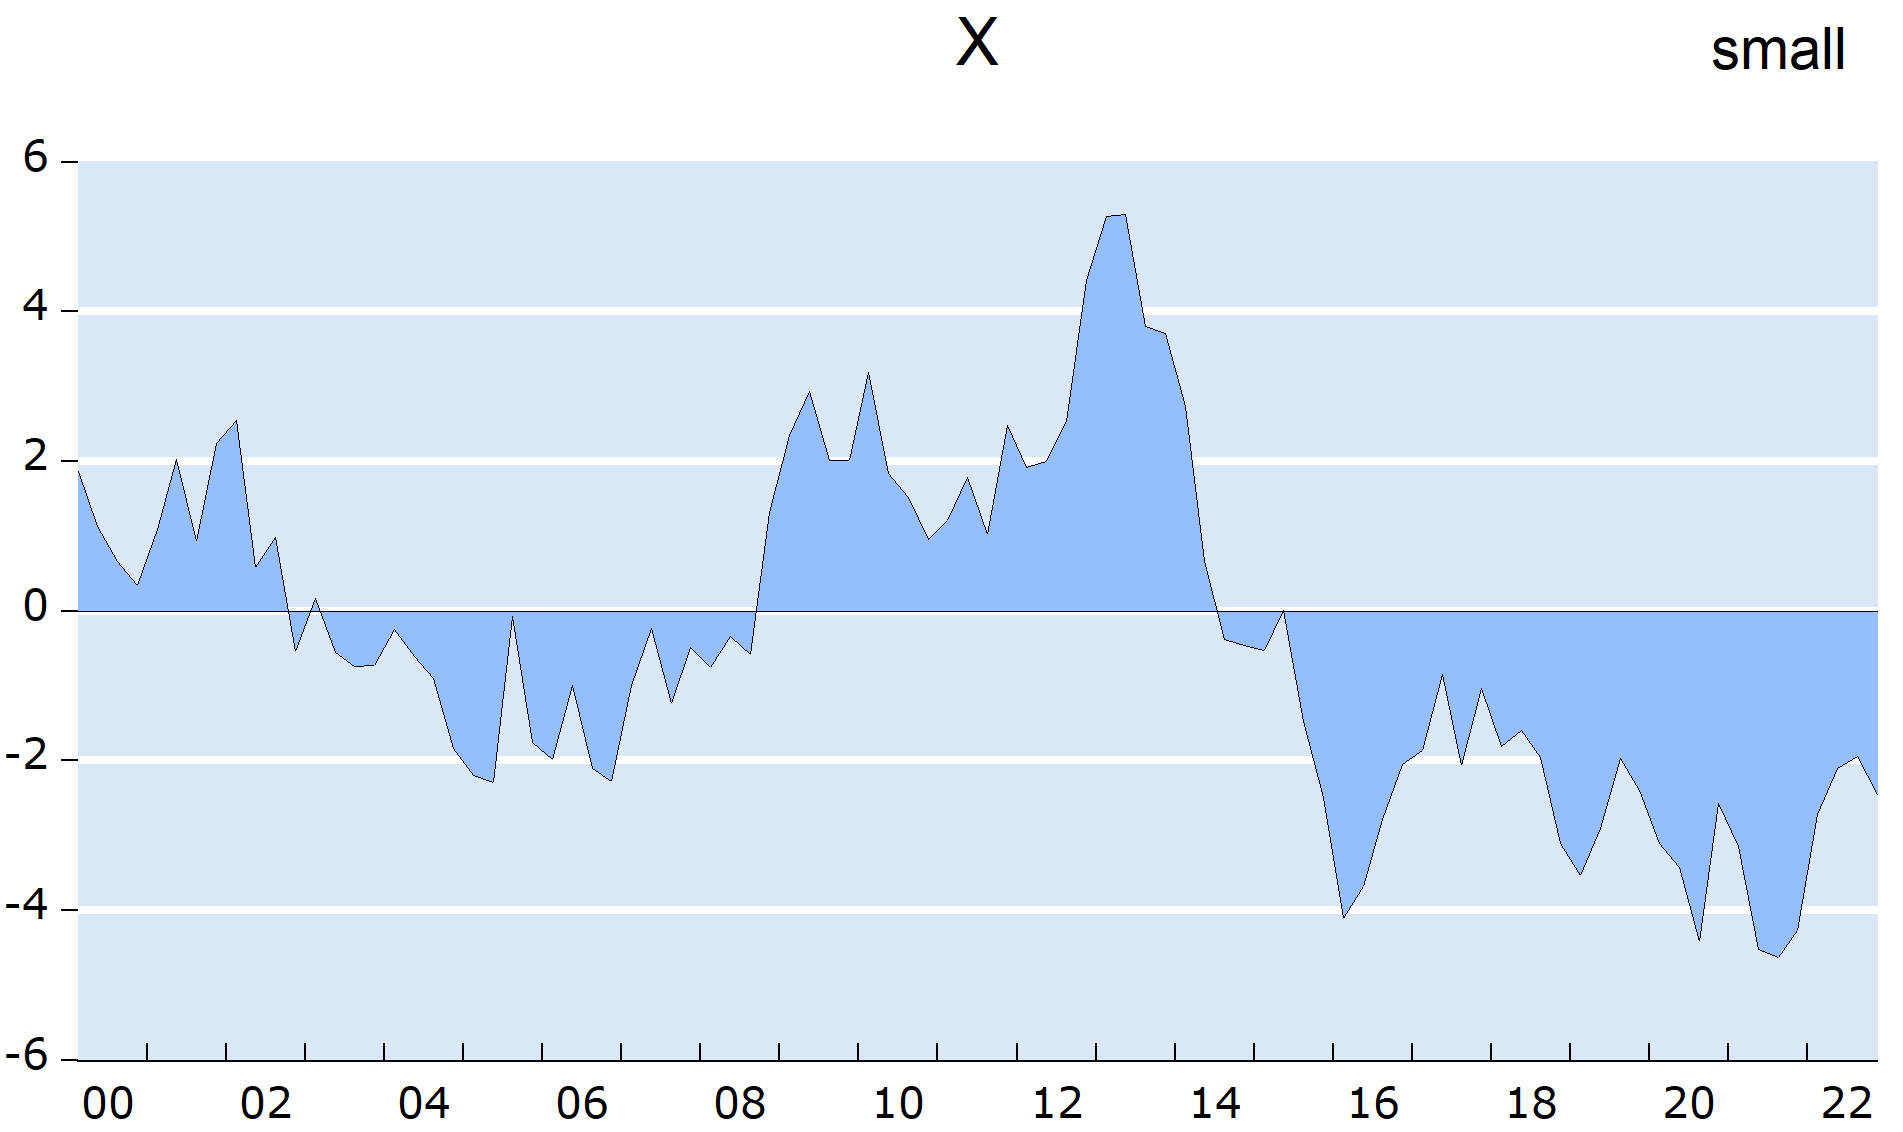
\includegraphics[width=0.33\textwidth,height=0.25\textwidth]{saniya-small-sag1} }\subfloat[Figure 2 of EviewsR page\label{fig:saniya-2}]{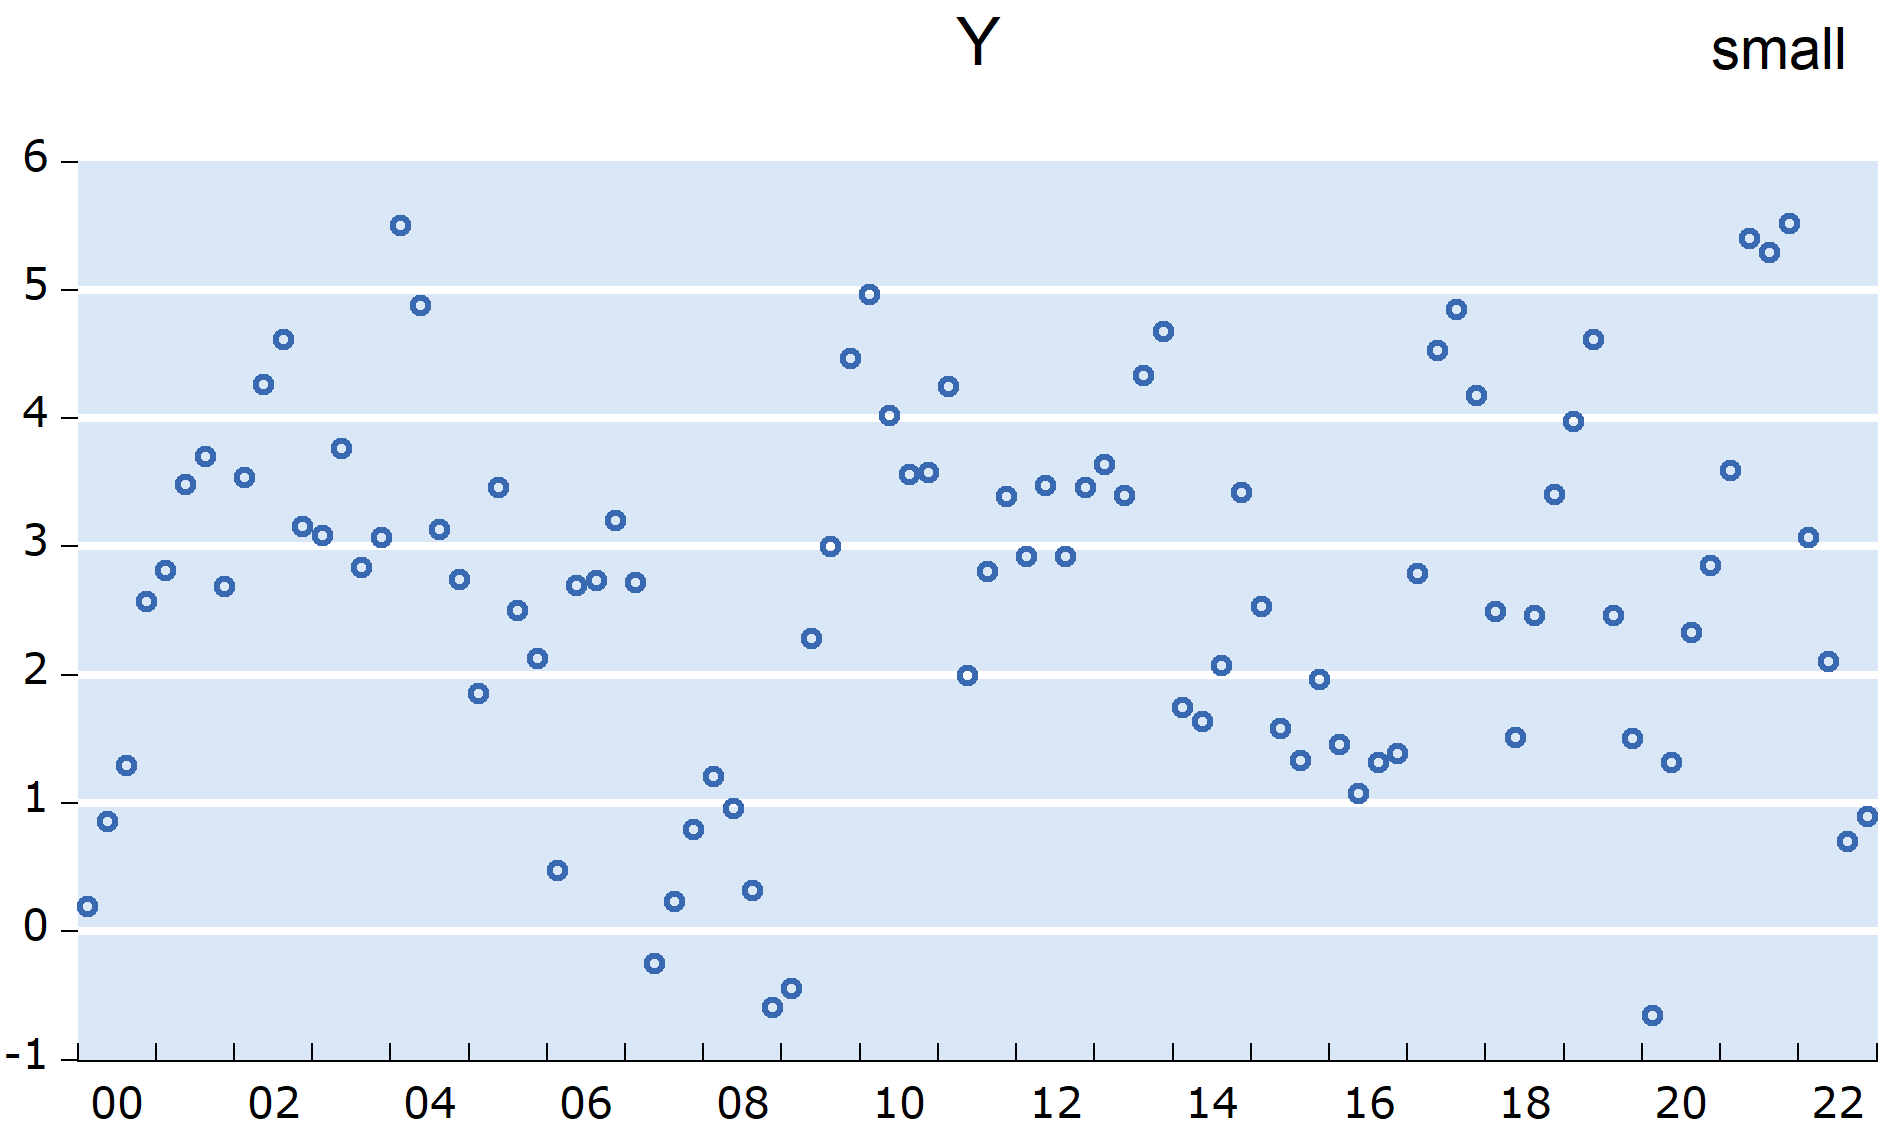
\includegraphics[width=0.33\textwidth,height=0.25\textwidth]{saniya-small-sag2} }\subfloat[Figure 3 of EviewsR page\label{fig:saniya-3}]{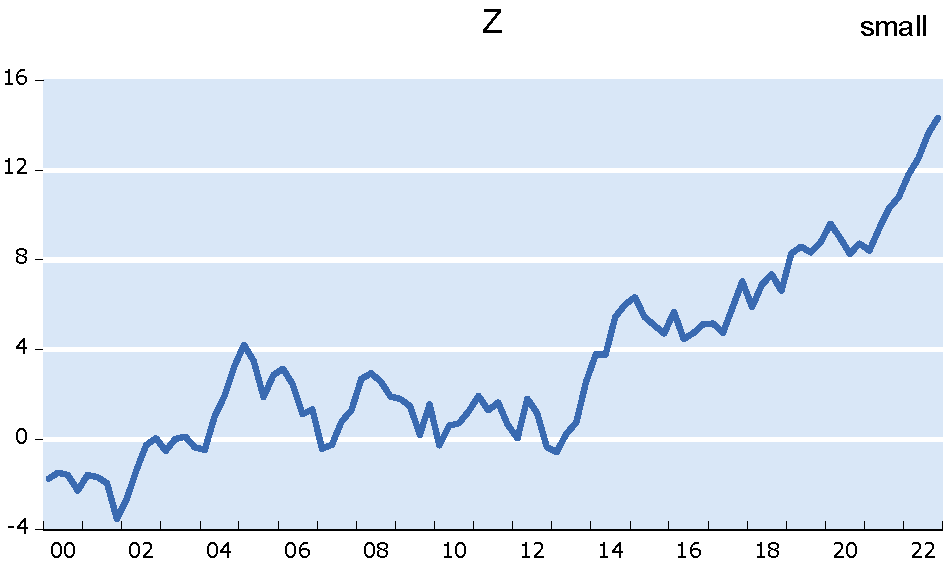
\includegraphics[width=0.33\textwidth,height=0.25\textwidth]{saniya-small-sag3} }\caption{Figures import}\label{fig:saniya}
\end{figure}

\begin{Shaded}
\begin{Highlighting}[]
\SpecialCharTok{\textgreater{}} \FunctionTok{library}\NormalTok{(magrittr)}
\SpecialCharTok{\textgreater{}} 
\ErrorTok{\textgreater{}}\NormalTok{ a}\OtherTok{=}\FunctionTok{runif}\NormalTok{(}\DecValTok{100}\NormalTok{) }\SpecialCharTok{\%\textgreater{}\%}\NormalTok{ plot}
\SpecialCharTok{\textgreater{}}\NormalTok{ a}\OtherTok{=}\FunctionTok{runif}\NormalTok{(}\DecValTok{100}\NormalTok{) }\SpecialCharTok{\%\textgreater{}\%}\NormalTok{ plot}
\SpecialCharTok{\textgreater{}}\NormalTok{ a}\OtherTok{=}\FunctionTok{runif}\NormalTok{(}\DecValTok{100}\NormalTok{) }\SpecialCharTok{\%\textgreater{}\%}\NormalTok{ plot}
\SpecialCharTok{\textgreater{}}\NormalTok{ a}\OtherTok{=}\FunctionTok{runif}\NormalTok{(}\DecValTok{100}\NormalTok{) }\SpecialCharTok{\%\textgreater{}\%}\NormalTok{ plot}
\SpecialCharTok{\textgreater{}}\NormalTok{ a}\OtherTok{=}\FunctionTok{runif}\NormalTok{(}\DecValTok{100}\NormalTok{) }\SpecialCharTok{\%\textgreater{}\%}\NormalTok{ plot}
\SpecialCharTok{\textgreater{}}\NormalTok{ a}\OtherTok{=}\FunctionTok{runif}\NormalTok{(}\DecValTok{100}\NormalTok{) }\SpecialCharTok{\%\textgreater{}\%}\NormalTok{ plot}
\SpecialCharTok{\textgreater{}}\NormalTok{ a}\OtherTok{=}\FunctionTok{runif}\NormalTok{(}\DecValTok{100}\NormalTok{) }\SpecialCharTok{\%\textgreater{}\%}\NormalTok{ plot}
\SpecialCharTok{\textgreater{}}\NormalTok{ a}\OtherTok{=}\FunctionTok{runif}\NormalTok{(}\DecValTok{100}\NormalTok{) }\SpecialCharTok{\%\textgreater{}\%}\NormalTok{ plot}
\SpecialCharTok{\textgreater{}}\NormalTok{ a}\OtherTok{=}\FunctionTok{runif}\NormalTok{(}\DecValTok{100}\NormalTok{) }\SpecialCharTok{\%\textgreater{}\%}\NormalTok{ plot}
\end{Highlighting}
\end{Shaded}

\begin{figure}[h]
\subfloat[1\label{fig:unnamed-chunk-1-1}]{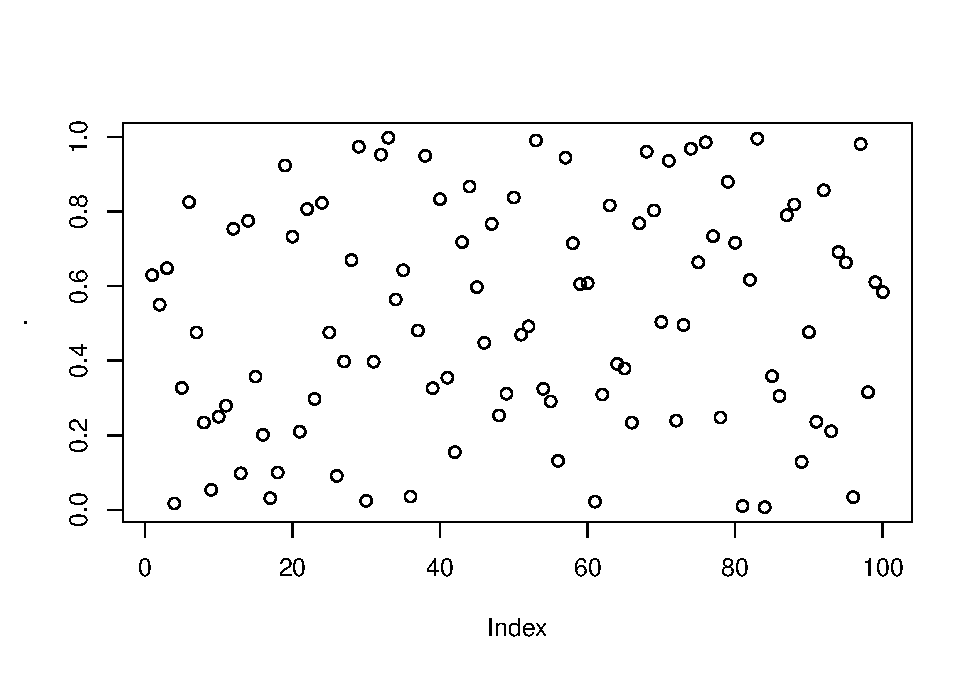
\includegraphics[width=0.33\textwidth]{eviews_graphs_files/figure-latex/unnamed-chunk-1-1} }\subfloat[2\label{fig:unnamed-chunk-1-2}]{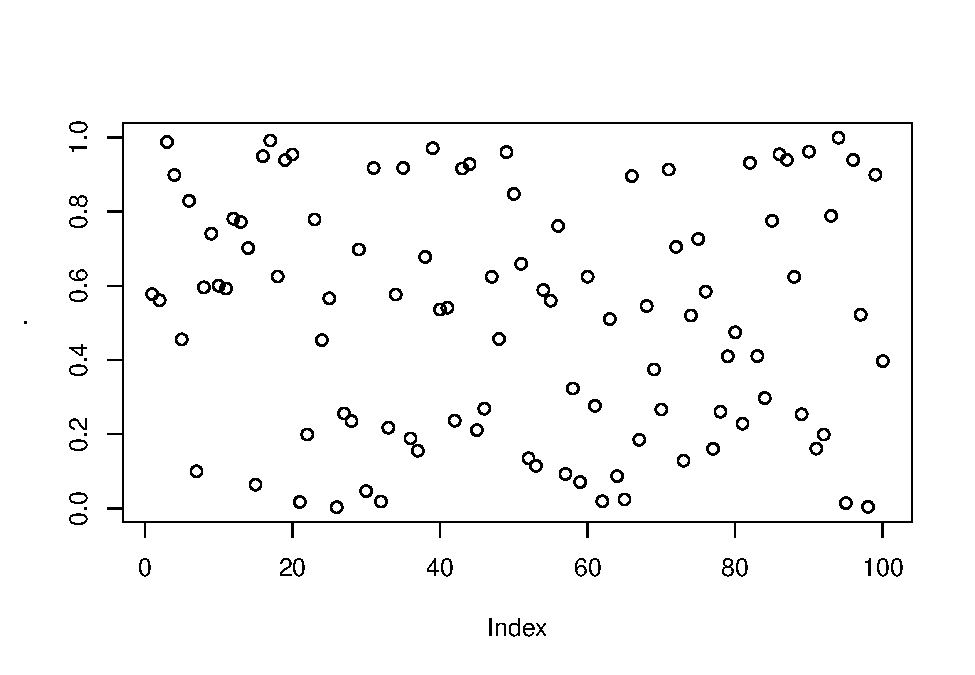
\includegraphics[width=0.33\textwidth]{eviews_graphs_files/figure-latex/unnamed-chunk-1-2} }\subfloat[3\label{fig:unnamed-chunk-1-3}]{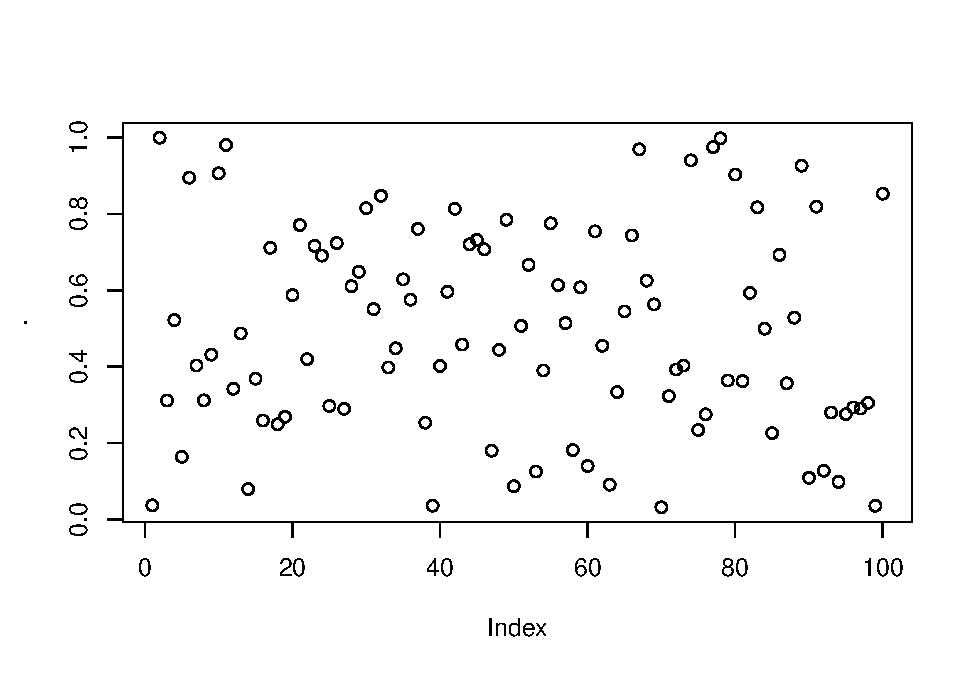
\includegraphics[width=0.33\textwidth]{eviews_graphs_files/figure-latex/unnamed-chunk-1-3} }\newline\subfloat[4\label{fig:unnamed-chunk-1-4}]{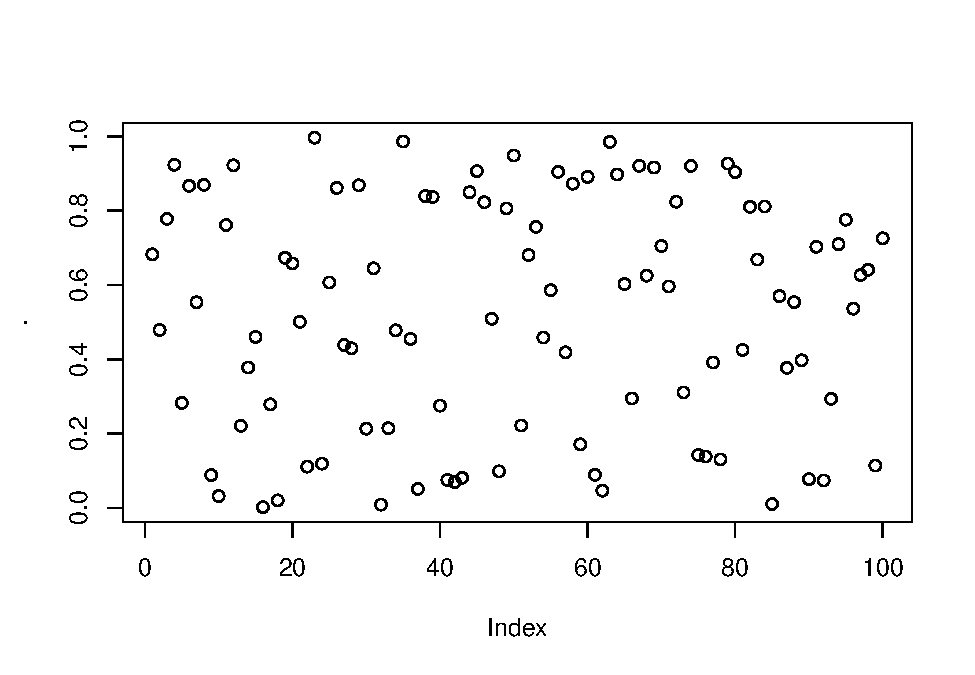
\includegraphics[width=0.33\textwidth]{eviews_graphs_files/figure-latex/unnamed-chunk-1-4} }\subfloat[5\label{fig:unnamed-chunk-1-5}]{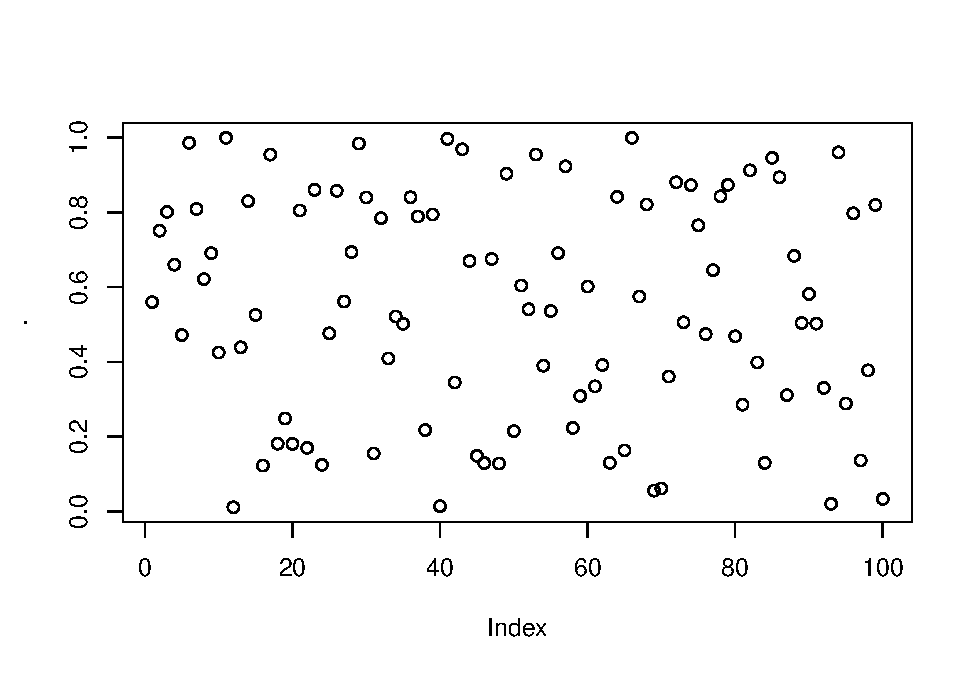
\includegraphics[width=0.33\textwidth]{eviews_graphs_files/figure-latex/unnamed-chunk-1-5} }\subfloat[6\label{fig:unnamed-chunk-1-6}]{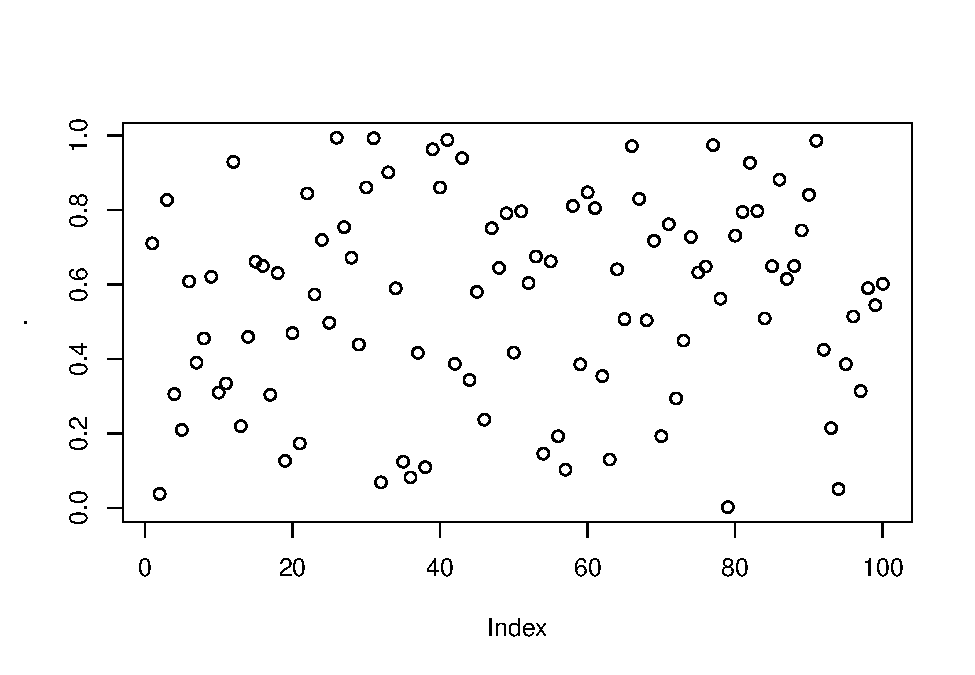
\includegraphics[width=0.33\textwidth]{eviews_graphs_files/figure-latex/unnamed-chunk-1-6} }\newline\subfloat[7\label{fig:unnamed-chunk-1-7}]{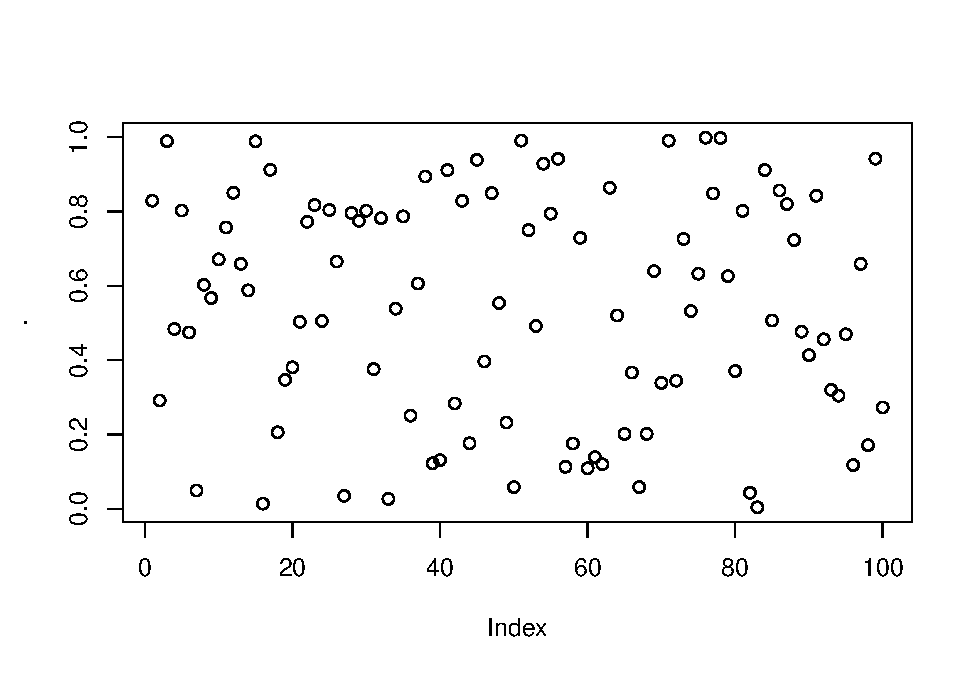
\includegraphics[width=0.33\textwidth]{eviews_graphs_files/figure-latex/unnamed-chunk-1-7} }\subfloat[8\label{fig:unnamed-chunk-1-8}]{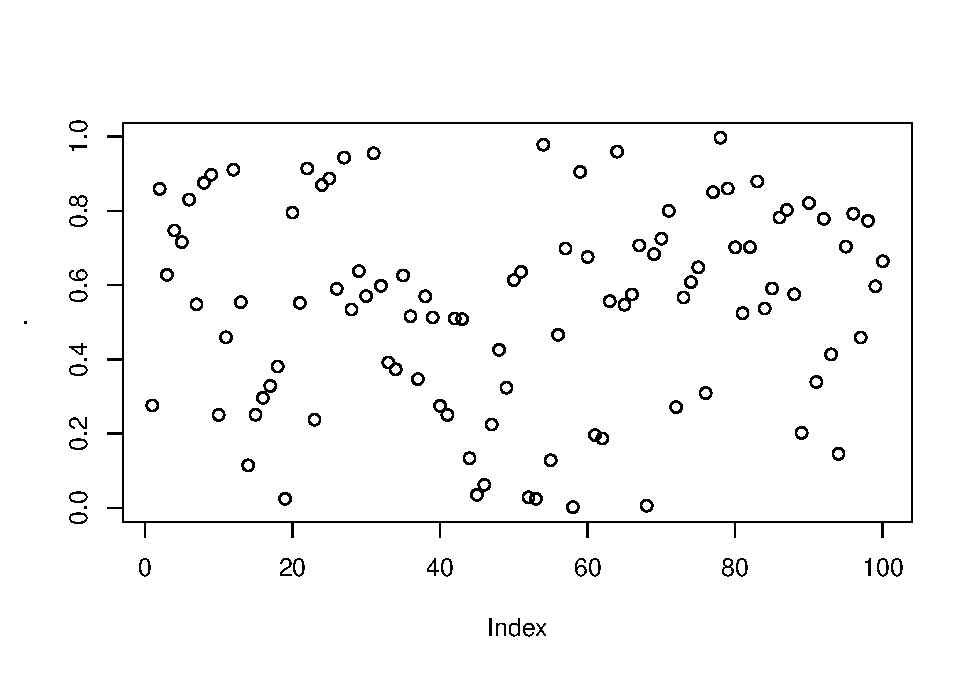
\includegraphics[width=0.33\textwidth]{eviews_graphs_files/figure-latex/unnamed-chunk-1-8} }\subfloat[9\label{fig:unnamed-chunk-1-9}]{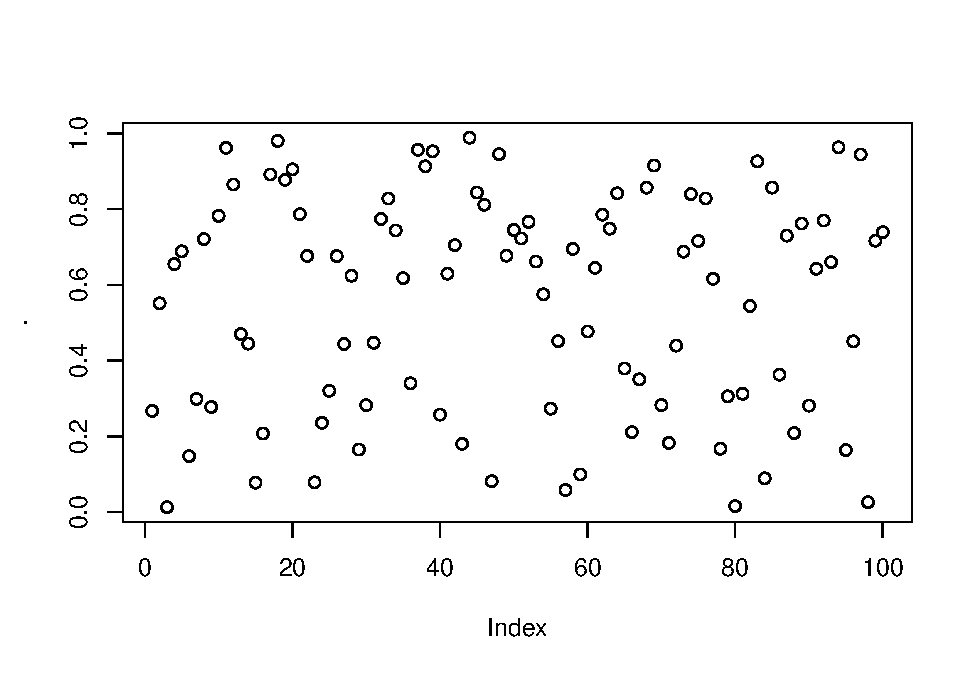
\includegraphics[width=0.33\textwidth]{eviews_graphs_files/figure-latex/unnamed-chunk-1-9} }\caption{some plot again}\label{fig:unnamed-chunk-1}
\end{figure}

\begin{Shaded}
\begin{Highlighting}[]
\SpecialCharTok{\textgreater{}} \FunctionTok{library}\NormalTok{(magrittr)}
\SpecialCharTok{\textgreater{}} 
\ErrorTok{\textgreater{}}\NormalTok{ a}\OtherTok{=}\FunctionTok{runif}\NormalTok{(}\DecValTok{100}\NormalTok{) }\SpecialCharTok{\%\textgreater{}\%}\NormalTok{ plot}
\SpecialCharTok{\textgreater{}}\NormalTok{ a}\OtherTok{=}\FunctionTok{runif}\NormalTok{(}\DecValTok{100}\NormalTok{) }\SpecialCharTok{\%\textgreater{}\%}\NormalTok{ plot}
\SpecialCharTok{\textgreater{}}\NormalTok{ a}\OtherTok{=}\FunctionTok{runif}\NormalTok{(}\DecValTok{100}\NormalTok{) }\SpecialCharTok{\%\textgreater{}\%}\NormalTok{ plot}
\SpecialCharTok{\textgreater{}}\NormalTok{ a}\OtherTok{=}\FunctionTok{runif}\NormalTok{(}\DecValTok{100}\NormalTok{) }\SpecialCharTok{\%\textgreater{}\%}\NormalTok{ plot}
\SpecialCharTok{\textgreater{}}\NormalTok{ a}\OtherTok{=}\FunctionTok{runif}\NormalTok{(}\DecValTok{100}\NormalTok{) }\SpecialCharTok{\%\textgreater{}\%}\NormalTok{ plot}
\SpecialCharTok{\textgreater{}}\NormalTok{ a}\OtherTok{=}\FunctionTok{runif}\NormalTok{(}\DecValTok{100}\NormalTok{) }\SpecialCharTok{\%\textgreater{}\%}\NormalTok{ plot}
\SpecialCharTok{\textgreater{}}\NormalTok{ a}\OtherTok{=}\FunctionTok{runif}\NormalTok{(}\DecValTok{100}\NormalTok{) }\SpecialCharTok{\%\textgreater{}\%}\NormalTok{ plot}
\SpecialCharTok{\textgreater{}}\NormalTok{ a}\OtherTok{=}\FunctionTok{runif}\NormalTok{(}\DecValTok{100}\NormalTok{) }\SpecialCharTok{\%\textgreater{}\%}\NormalTok{ plot}
\SpecialCharTok{\textgreater{}}\NormalTok{ a}\OtherTok{=}\FunctionTok{runif}\NormalTok{(}\DecValTok{100}\NormalTok{) }\SpecialCharTok{\%\textgreater{}\%}\NormalTok{ plot}
\end{Highlighting}
\end{Shaded}

\begin{figure}[h]
\subfloat[1\label{fig:unnamed-chunk-2-1}]{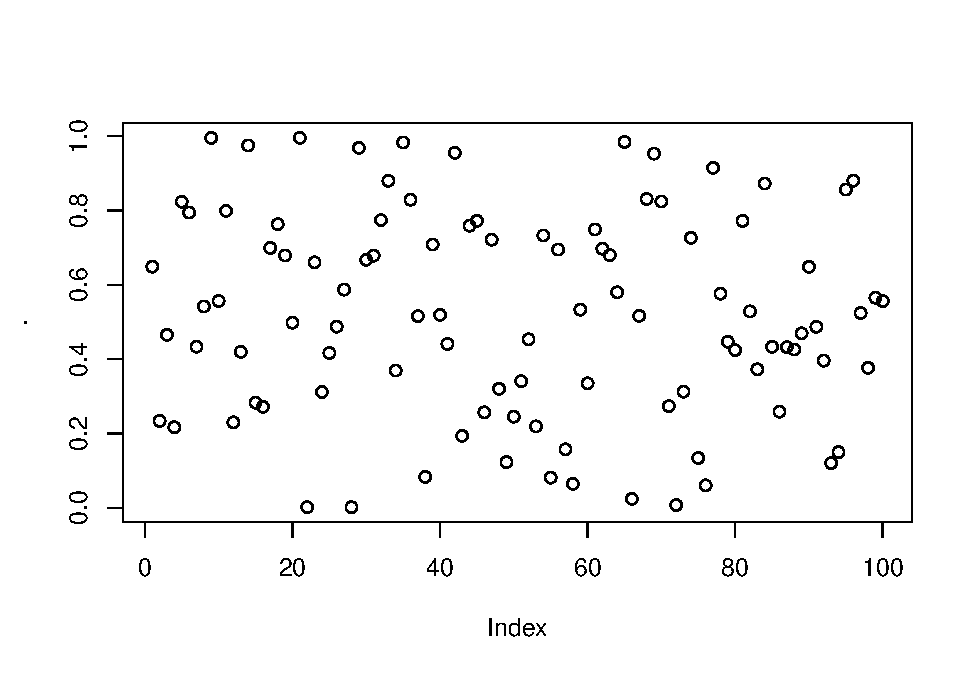
\includegraphics[width=0.33\textwidth]{eviews_graphs_files/figure-latex/unnamed-chunk-2-1} }\subfloat[2\label{fig:unnamed-chunk-2-2}]{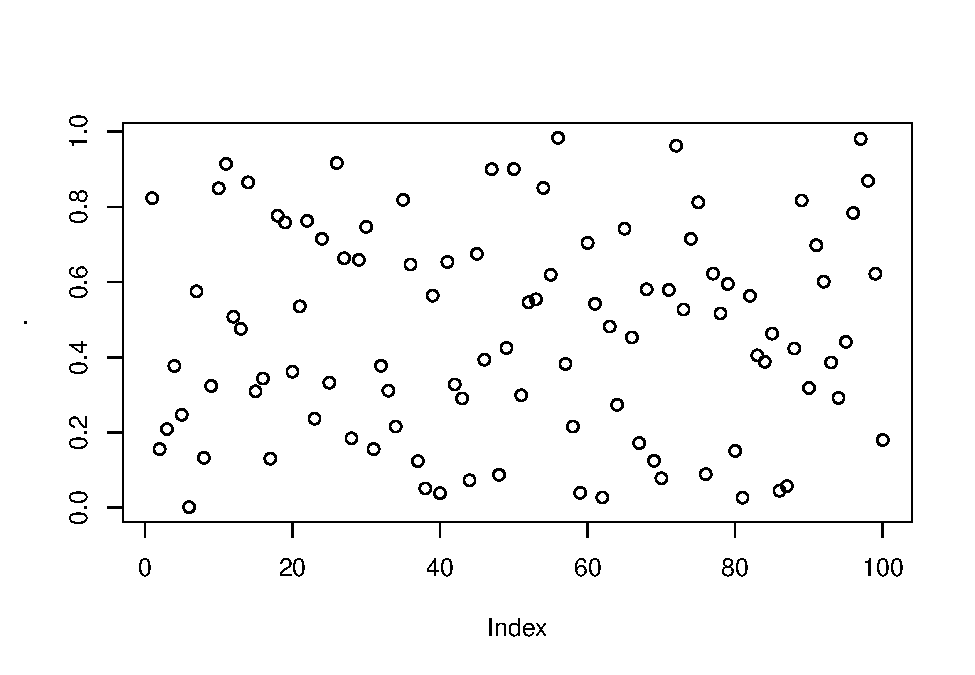
\includegraphics[width=0.33\textwidth]{eviews_graphs_files/figure-latex/unnamed-chunk-2-2} }\subfloat[3\label{fig:unnamed-chunk-2-3}]{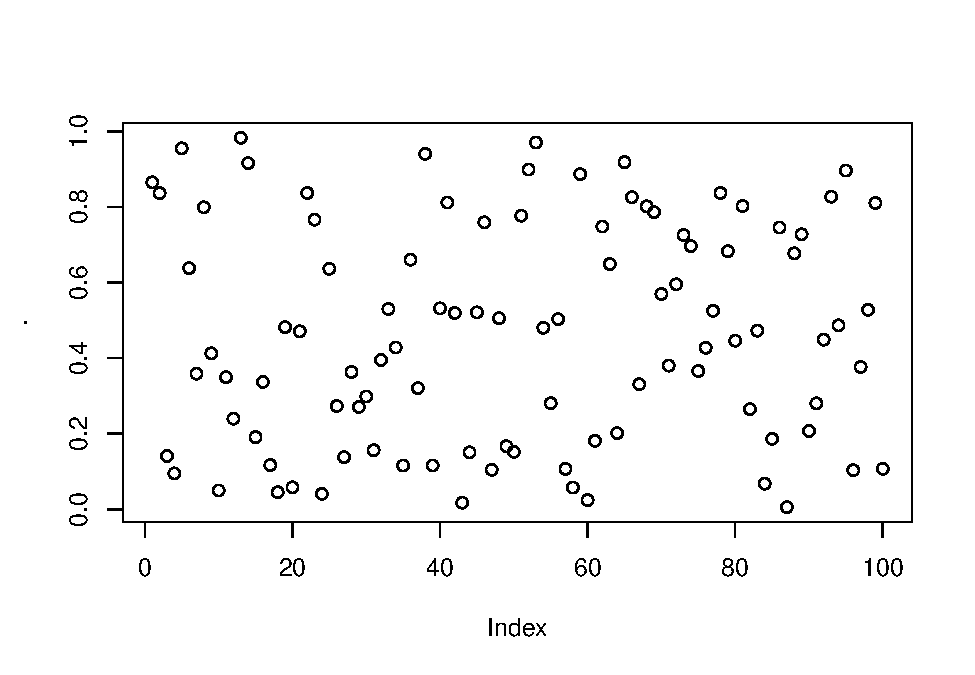
\includegraphics[width=0.33\textwidth]{eviews_graphs_files/figure-latex/unnamed-chunk-2-3} }\newline\subfloat[4\label{fig:unnamed-chunk-2-4}]{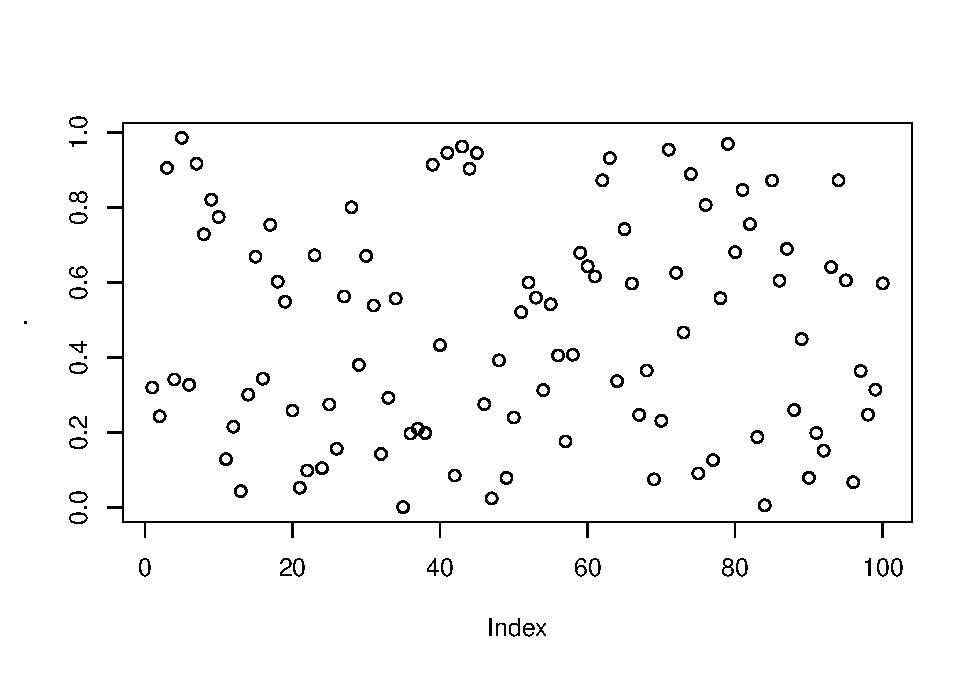
\includegraphics[width=0.33\textwidth]{eviews_graphs_files/figure-latex/unnamed-chunk-2-4} }\subfloat[5\label{fig:unnamed-chunk-2-5}]{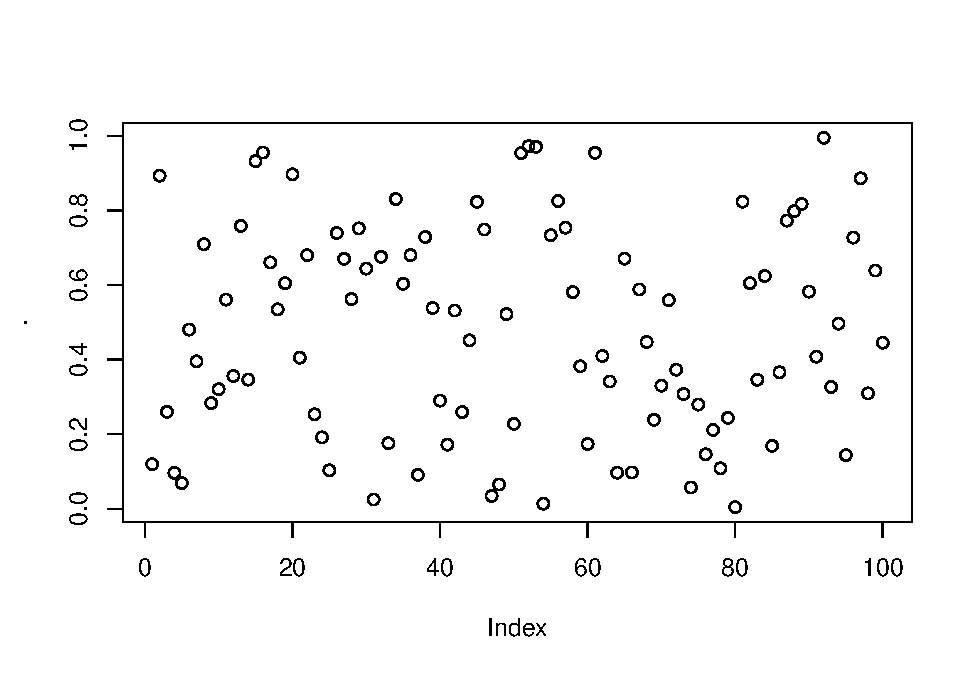
\includegraphics[width=0.33\textwidth]{eviews_graphs_files/figure-latex/unnamed-chunk-2-5} }\subfloat[6\label{fig:unnamed-chunk-2-6}]{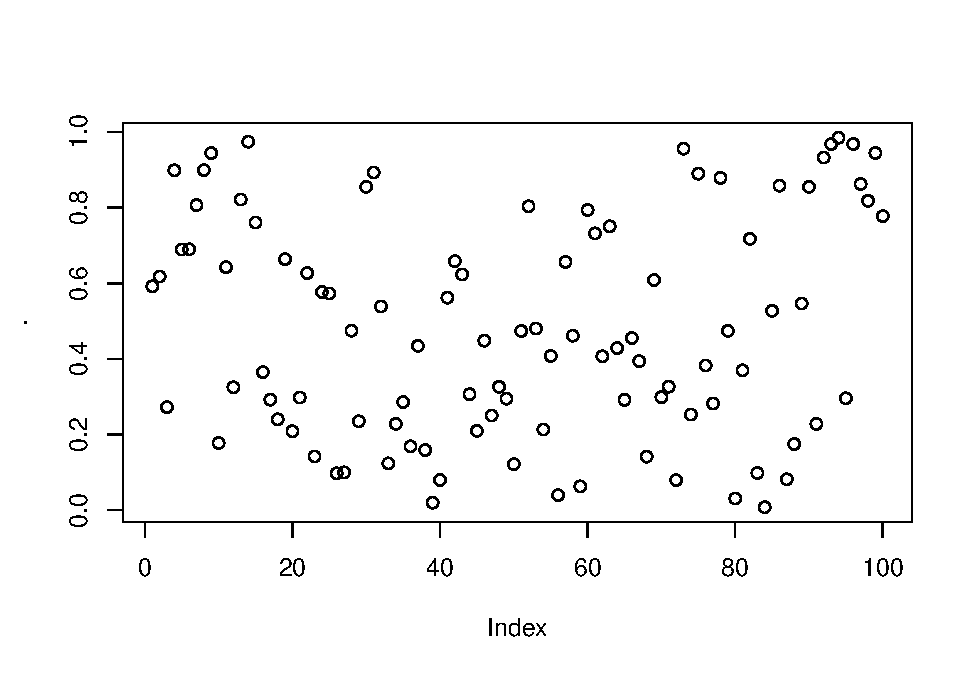
\includegraphics[width=0.33\textwidth]{eviews_graphs_files/figure-latex/unnamed-chunk-2-6} }\newline\subfloat[7\label{fig:unnamed-chunk-2-7}]{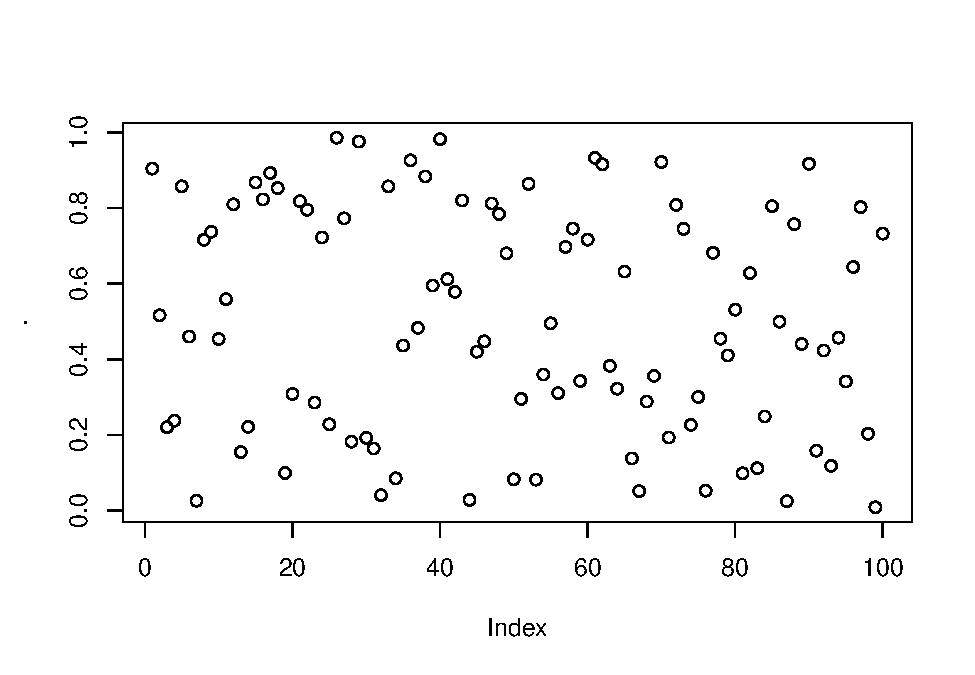
\includegraphics[width=0.33\textwidth]{eviews_graphs_files/figure-latex/unnamed-chunk-2-7} }\subfloat[8\label{fig:unnamed-chunk-2-8}]{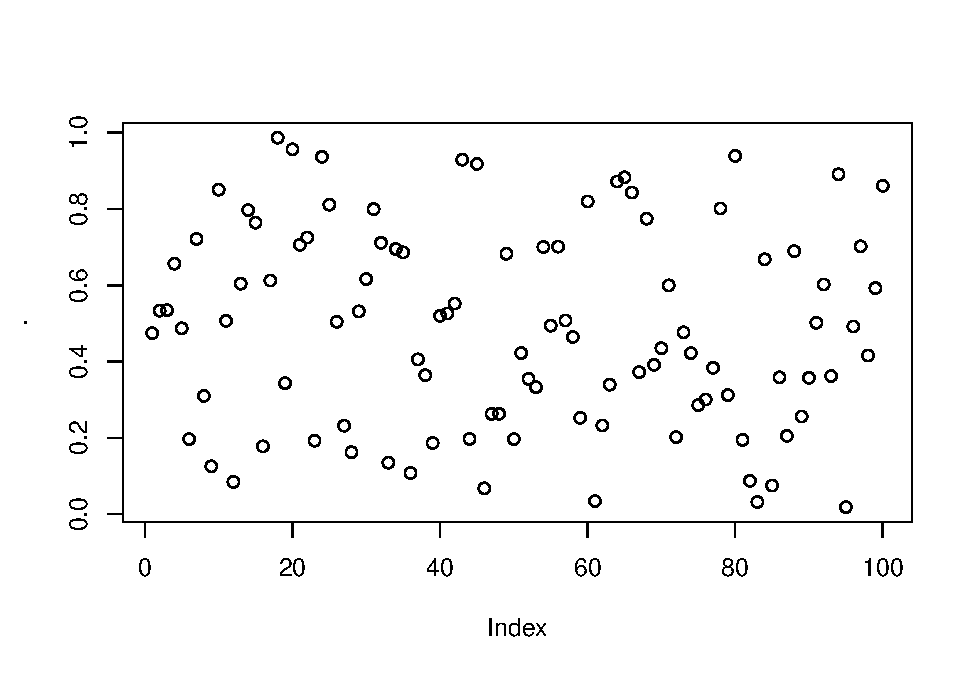
\includegraphics[width=0.33\textwidth]{eviews_graphs_files/figure-latex/unnamed-chunk-2-8} }\subfloat[9\label{fig:unnamed-chunk-2-9}]{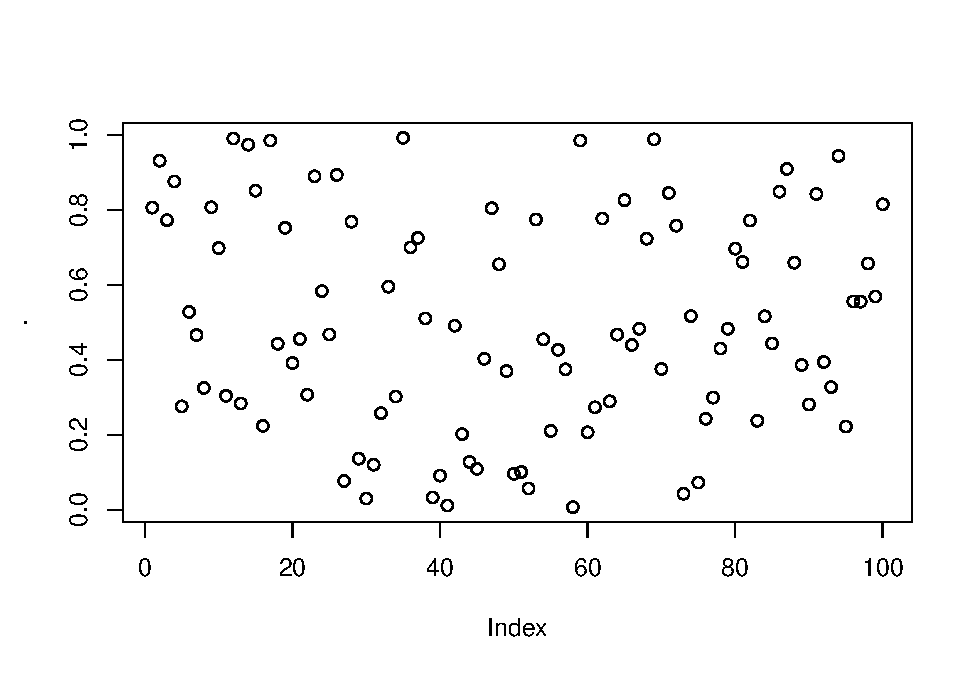
\includegraphics[width=0.33\textwidth]{eviews_graphs_files/figure-latex/unnamed-chunk-2-9} }\caption{some plot}\label{fig:unnamed-chunk-2}
\end{figure}

\begin{figure}[h]
\subfloat[Figure 1 of EviewsR page\label{fig:biscuit-1}]{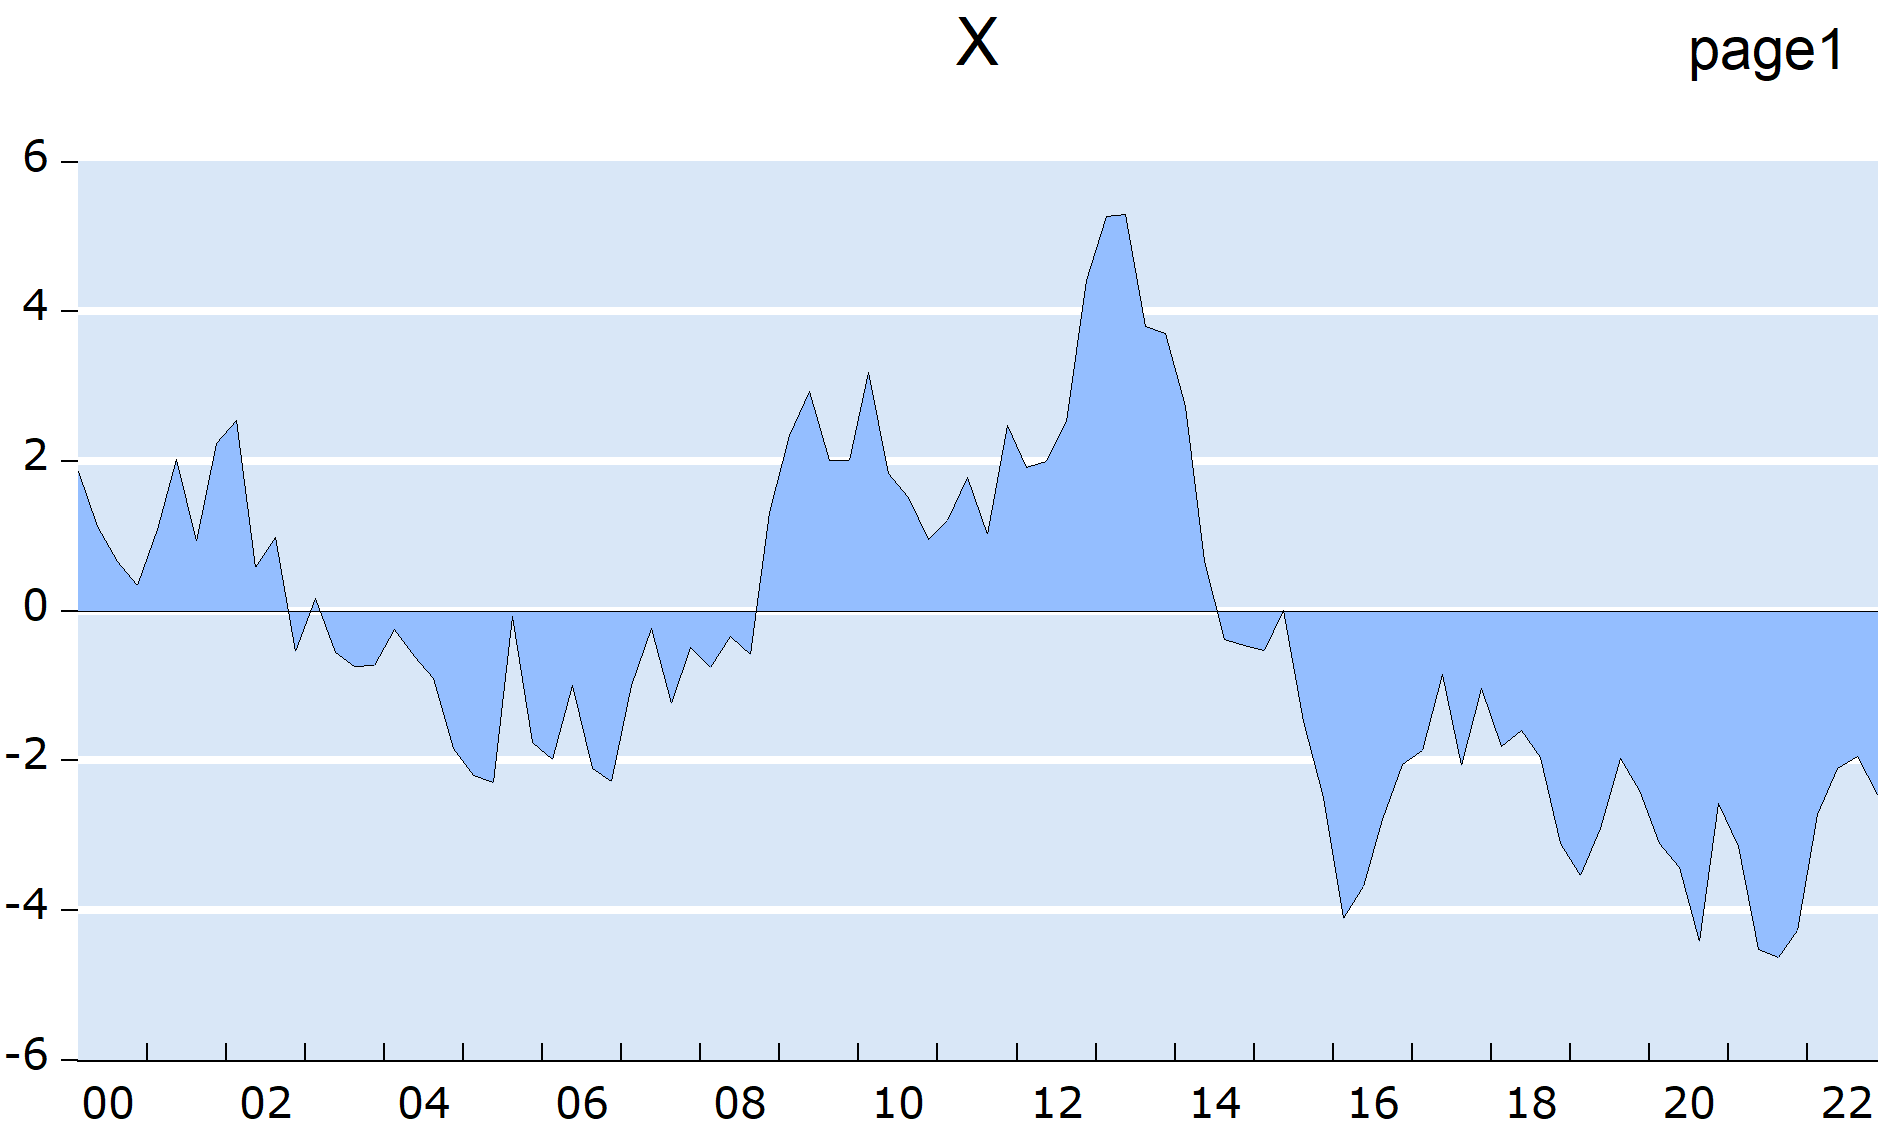
\includegraphics[width=0.33\textwidth,height=0.25\textwidth]{biscuit-page1-graph1} }\subfloat[Figure 2 of EviewsR page\label{fig:biscuit-2}]{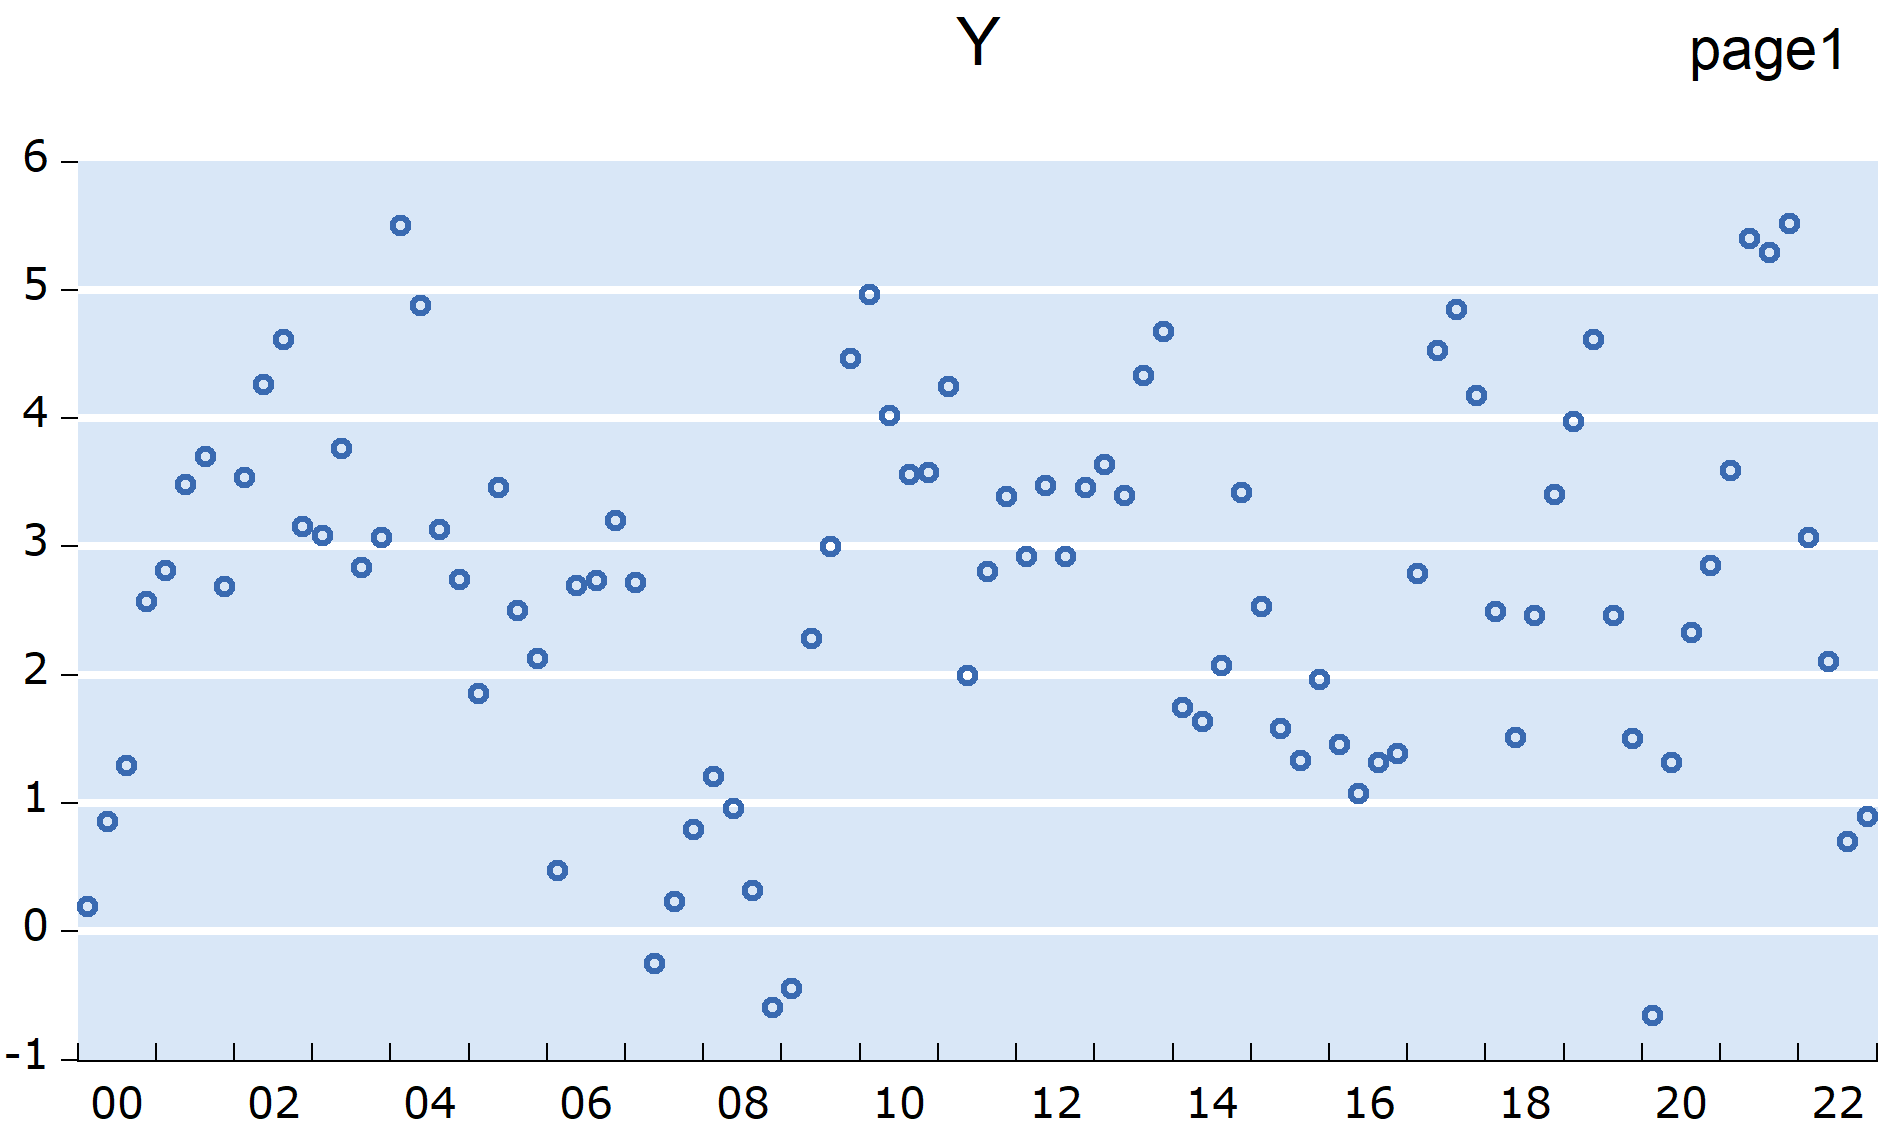
\includegraphics[width=0.33\textwidth,height=0.25\textwidth]{biscuit-page1-graph2} }\subfloat[Figure 3 of EviewsR page\label{fig:biscuit-3}]{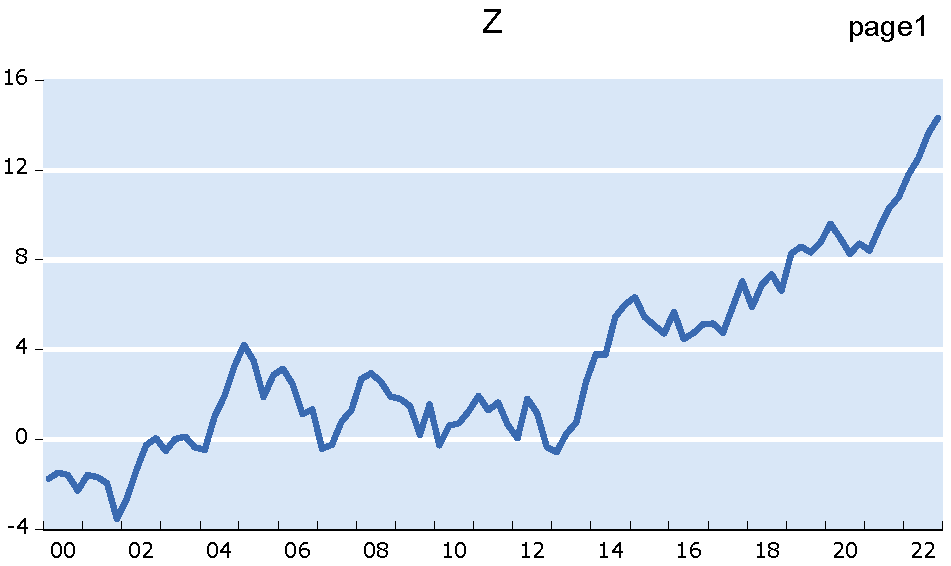
\includegraphics[width=0.33\textwidth,height=0.25\textwidth]{biscuit-page1-graph3} }\newline\subfloat[Figure 1 of Page1 page\label{fig:biscuit-4}]{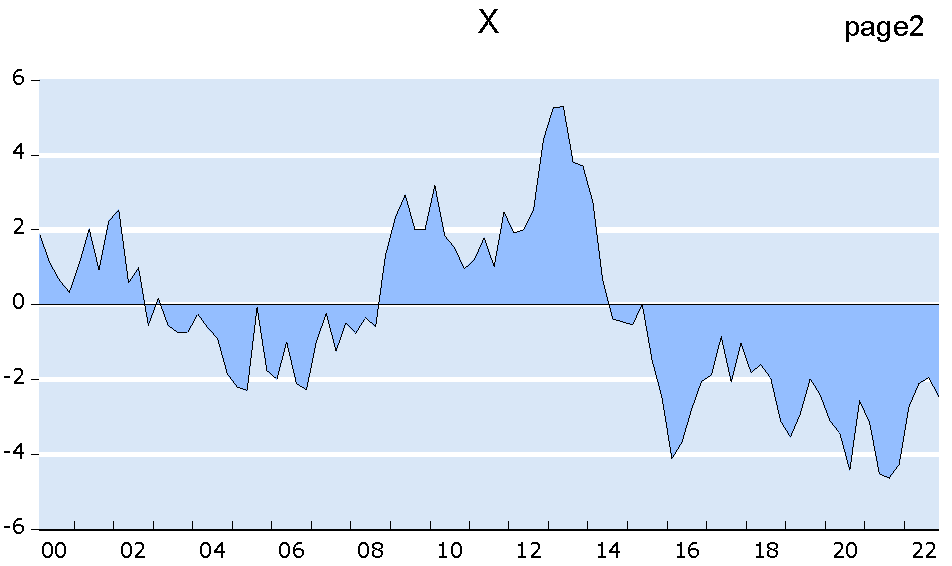
\includegraphics[width=0.33\textwidth,height=0.25\textwidth]{biscuit-page2-graph1} }\subfloat[Figure 2 of Page1 page\label{fig:biscuit-5}]{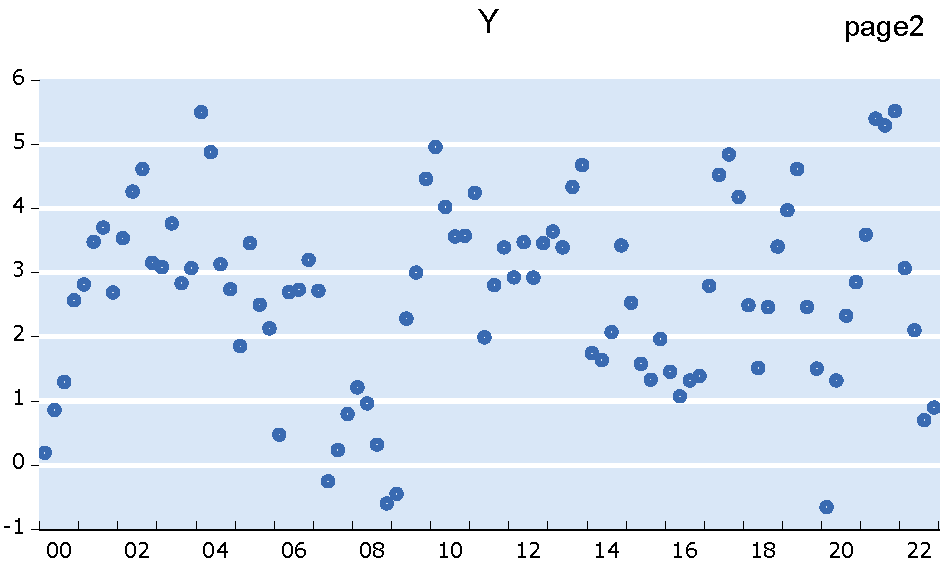
\includegraphics[width=0.33\textwidth,height=0.25\textwidth]{biscuit-page2-graph2} }\subfloat[Figure 3 of Page1 page\label{fig:biscuit-6}]{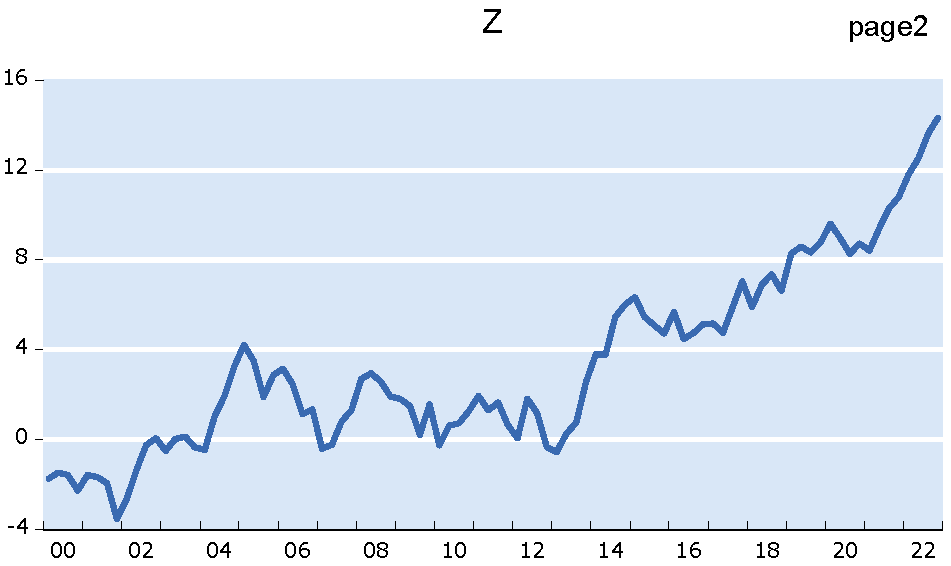
\includegraphics[width=0.33\textwidth,height=0.25\textwidth]{biscuit-page2-graph3} }\caption{Figures automatically imported by eviews 2}\label{fig:biscuit}
\end{figure}

\begin{Shaded}
\begin{Highlighting}[]
\NormalTok{\textgreater{} /{-}{-}{-}{-}\textbackslash{} /{-}{-}{-}{-}\textbackslash{}}
\NormalTok{+ |c33F| |cC02|}
\NormalTok{+ |    | |    |}
\NormalTok{+ \textbackslash{}{-}{-}{-}{-}/ \textbackslash{}{-}{-}{-}{-}/}
\NormalTok{+ }
\NormalTok{+ /{-}{-}{-}{-}\textbackslash{} /{-}{-}{-}{-}\textbackslash{}}
\NormalTok{+ |c1FF| |c1AB|}
\NormalTok{+ |    | |    |}
\NormalTok{+ \textbackslash{}{-}{-}{-}{-}/ \textbackslash{}{-}{-}{-}{-}/}
\end{Highlighting}
\end{Shaded}

\begin{Shaded}
\begin{Highlighting}[]
\SpecialCharTok{\textgreater{}}\NormalTok{ x}\OtherTok{=}\FunctionTok{cumsum}\NormalTok{(}\FunctionTok{rnorm}\NormalTok{(}\DecValTok{100}\NormalTok{))}
\SpecialCharTok{\textgreater{}}\NormalTok{ y}\OtherTok{=}\FunctionTok{cumsum}\NormalTok{(}\FunctionTok{rnorm}\NormalTok{(}\DecValTok{100}\NormalTok{))}
\SpecialCharTok{\textgreater{}}\NormalTok{ z}\OtherTok{=}\FunctionTok{cumsum}\NormalTok{(}\FunctionTok{rnorm}\NormalTok{(}\DecValTok{100}\NormalTok{))}
\SpecialCharTok{\textgreater{}}\NormalTok{ data}\OtherTok{=}\FunctionTok{data.frame}\NormalTok{(x,y,z)}
\SpecialCharTok{\textgreater{}} \FunctionTok{eviews\_graph}\NormalTok{(data,}\AttributeTok{group =}\NormalTok{ T,}\AttributeTok{options =} \StringTok{\textquotesingle{}m\textquotesingle{}}\NormalTok{)}
\end{Highlighting}
\end{Shaded}

\begin{figure}[h]
\includegraphics[width=\textwidth]{eviews_graphs_files/figure-latex//graphp-graphp-XYZ} \caption{Nice graph}\label{fig:graphp}
\end{figure}

\end{document}
